\subsection{The controller}
\label{sec:ppcontroller}

\begin{figure}
\centering
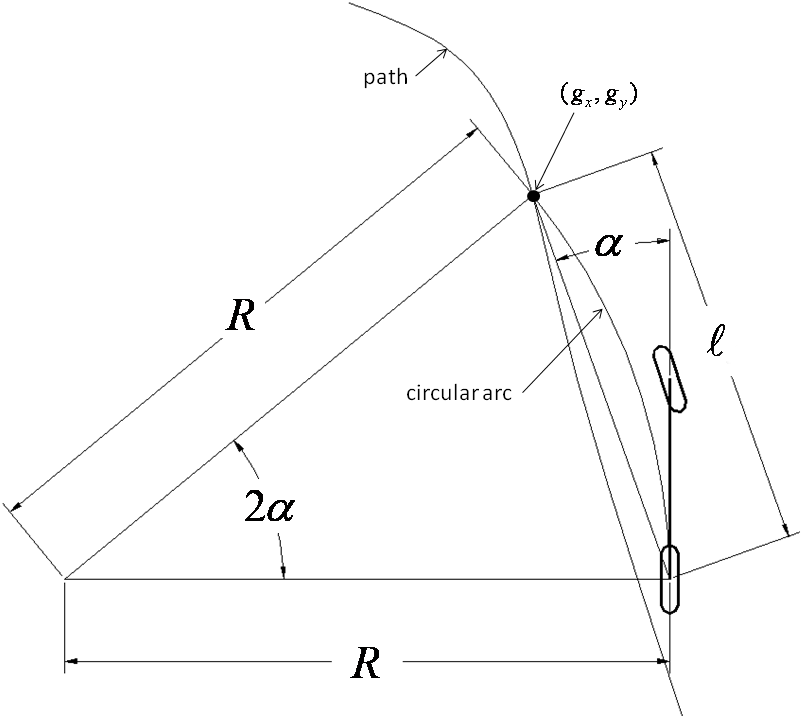
\includegraphics[width=50mm]{Figures/Purepursuit.png}%
\caption{Purepursuit path-tracking \cite{Snider.2009}.}
\label{fig:purepursuit}%
\end{figure}

The path given by the planner is tracked using the pure-pursuit controller~\cite{Amidi.1991}
as formulated in~\cite{Snider.2009}.
%
The path is described in the car's \emph{rear-axle coordinates}.
%
The origin of the rear axle coordinates is the center of the rear axle, the x-axis is the heading of the car, and the heading of the y-axis is 90 degrees counterclockwise from the x-axis.
%
The output of the controller is the steering angle $\delta$ of the car.
%
The controller chooses a \emph{goal} point on the tracking path to determine the steering angle.
%
This point is chosen at a fixed distance from the rear axle, the \emph{lookahead distance}.
%
Let $(g_x, g_y)$ be the coordinates of the goal point in the rear-axle frame.
%
Note that the lookahead distance $\ell$ is $\sqrt{g_x^2+g_y^2}$.
%
If $L$ is the \emph{wheelbase} of the car (i.e. distance between rear and front axles), then the pure-pursuit steering angle $\delta$ is
\begin{align}
\delta & = tan^{-1}(\frac{2Lsin(\alpha)}{\ell}) \nonumber \\
 & =  tan^{-1}(\frac{2L g_y}{\ell^2})
 \label{eqn:purepursuit}
\end{align}
%
See Figure \ref{fig:purepursuit}.
%
This formula is valid only when $g_x > 0$
i.e. when the goal point is on the front of the rear axle.
%
In this case,
we have $\frac{-\pi}{2} < \delta < \frac{\pi}{2} $.